%%%%%%%%%%%%%%%%%%%%%%%%%%%%%%%%%%%%%%%%%%%%%%%%%%%%%%%%%%%%%%%%%%%%%%%%%%%%%%%%
%
% A Template for Trace Documents
% 
% This is a template for producing TRACE documents according to:
%
% Grimm V, Augusiak J, Focks A, Frank B, Gabsi F, Johnston ASA,  
% Liu C, Martin BT, Meli M, Radchuk V,  Thorbek P, Railsback SF. 2014. 
% Towards better modelling and decision support: documenting model development, 
%  testing, and analysis using TRACE. Ecological Modelling  
%
% and
%
% Augusiak J, Van den Brink PJ, Grimm V. 2014. Merging validation and evaluation of 
% ecological models to `evaludation': a review of terminology and a practical
%  approach. Ecological Modelling. 

% Before you compile a TRACE document, please read the above two publications, plus:

% Schmolke A, Thorbek P, DeAngelis DL, Grimm V. 2010. Ecological modelling supporting 
% environmental decision making: a strategy for the future. 
% Trends in Ecology and Evolution 25: 479-486.

% In the template, text in < > provides instructions and explanations and should be 
% replaced by your own text. By filling in your own text, tables, figures, and 
% hyperlinks, and by deleting instructions and explanations, you can create your 
% own TRACE document. 

% Please keep the short explanation that is given at the begin of each TRACE element; 
% it will remind you and readers what this element is about.

% We recommend keeping the simplistic formatting of this file so TRACE documents 
% produced by different authors not only use the same structure and terminology, 
% but also look similar, making it easier for model users to perceive TRACE as a 
% standard format.

% TRACE documents are designed to be supplementary material provided in electronic 
% and/or printed form to add credibility to your model and its results. Please refer 
% in your main article or report, where you present the model and its application, 
% to the TRACE document in the following way:

% ``In the Supplementary Material, we provide a TRACE document ("TRAnsparent and 
% Comprehensive model Evaludation''; Schmolke et al. 2010; Grimm et al. 2014; 
% Augusiak et al. 2014) containing evidence that our model was thoughtfully designed, 
% correctly implemented, thoroughly tested, well understood, and appropriately used 
% for its intended purpose. A summary of the TRACE document is given in Table <..>."

% It is important that you refer to those publications so that model users can check 
% whether you followed the standard defined in Grimm et al. (2014), that they 
% understand the rationale of TRACE (Schmolke et al. 2010) and of model evaludation 
% (Augusiak et al. 2014); it also allows the developers of TRACE to scan the 
% literature for consistent use of TRACE, which is important for future refinements.
% See also: http://cream-itn.eu/trace 
% When producing your TRACE document, delete this first page.

%% End of MS Word Template's first page
%%%%%%%%%%%%%%%%%%%%%%%%%%%%%%%%%%%%%%%%%%%%%%%%%%%%%%%%%%%%%%%%%%%%%%%%%%%%%%%%%%%%%%
%% 
%% This document template was created by Richard A. Erickson.
%% Please feel free to contact him with any suggestions, tips, or improvements.
%% He may be reached at raerickson@gmail.com
%% Note that this template is provided without warranty and as is. However, he would
%% gladly take suggestions for improvement and would be happy to collaborate on 
%% creating a .sty file or improving documentation for this template.  
%%
%% LaTeX notes, suggestions, and tips:
%% 0) This document assumes the user is familiar with LaTeX basics.
%% 1) The PDF produced by this does not exactly follow the Word template because 
%%    because some of the suggestions in the Word template are included as 
%%    comments in the LaTeX template. 
%% 2) Conversely to point 1, some directions were copied over directly from the Word 
%%    file and may not make sense with LaTeX.
%% 3) The optional sectional table of contents requires is only included for section 1.
%%    If you desire TOC for other sections, simply copy and paste this example code. 
%% 4) I would suggest using the url package to include url links.
%% 5) Recall the \label{} and \ref{} functions to reference objects within the code.
%% 6) You'll need to include figures with the figures environment. I do not provide examples
%%    Within this document.



\documentclass{article}[12pt]
\usepackage[letterpaper, margin=1in]{geometry} % used to set margins and specify page size
\usepackage{fancyhdr} % used to create headers 
\usepackage{titlesec} % Used to change section headers
\usepackage{titletoc} % needed for the sectional table of contents
\usepackage{url}
\usepackage{natbib} % Used for citations
\usepackage[nottoc]{tocbibind}
\usepackage{setspace}
\usepackage{graphicx}
\usepackage{subcaption}
\usepackage{tocloft}
\usepackage{parskip}
\usepackage{amsmath}
\usepackage{amssymb, mathtools}
\usepackage{topcapt, booktabs} % used for tables
\renewcommand{\cftsecleader}{\cftdotfill{\cftdotsep}}


\onehalfspacing

\titleformat{\section}
{{\titlerule[0.8pt]}\normalfont\Large\bfseries}{\thesection}{1em}{}[{\titlerule[0.8pt]}]

\setlength{\parindent}{0pt}

\pagestyle{fancy}
\fancyhf{}

\chead{TRACE document: Erickson et al. Spatial IPM}
\cfoot{\thepage}

\begin{document}

\begin{center}
\textbf{{\huge TRACE document}}
\end{center}

This is a TRACE documentation (``TRAnsparent and Comprehensive model Evaludation''), 
which provides supporting evidence that our model presented in:
\begin{center}
\textbf{Erickson RA, Eager EA, Long, KR,  Kocovsky PM, Glover D, et al. A spatially discrete, integral projection model and its application to invasive carps. Ecological Modelling.}
\end{center}
was thoughtfully designed, correctly implemented, thoroughly tested, well understood, and appropriately used for its intended purpose. 

 The rationale of this document follows: 
\begin{verse}
Schmolke A, Thorbek P, DeAngelis DL, Grimm V. 2010. Ecological modelling supporting environmental decision making: a strategy for the future. \textit{Trends in Ecology and Evolution} 25:479-486.
\end{verse}
and uses the updated standard terminology and document structure in:
\begin{verse}
Grimm V, Augusiak J, Focks A, Frank B, Gabsi F, Johnston, Liu C, Martin BT, Meli M, Radchuk V, Thorbek P, Railsback SF. 2014. Towards better modelling and decision support: documenting model development, testing, and analysis using TRACE. \textit{Ecological Modelling} 280:129-139
\end{verse}
and
\begin{verse}
Augusiak J, Van den Brink PJ, Grimm V. 2014. Merging validation and evaluation of ecological models to `evaludation': a review of terminology and a practical approach. \textit{Ecological Modelling}. 280:117-128
\end{verse}


\pagebreak

% \dominitoc % Initialization
\tableofcontents

\pagebreak
\section{Problem Formulation}
\textbf{This TRACE element provides supporting information on:} The decision-making context in which the model will be used; the types of model clients or stakeholders addressed; a precise specification of the question(s) that should be answered with the model, including a specification of necessary model outputs; and a statement of the domain of applicability of the model, including the extent of acceptable extrapolations. 

\textbf{Summary:}
\begin{verse}
\textbf{ 
Resource managers and ecologists often seek to understand and model spatial dynamics of invasive species.
These models can be applied to both the management of species (e.g., ``how many do we need to kill?'') and development new control methods (e.g., ``is approach \textit{X} a feasible tool that should be further developed?''). 
Furthermore, management activities often target organisms of a specific size (e.g., harvest may only target large fish or a barrier may limit the movement small fish but not large fish).
We developed a spatially explicit, integral projection model that can be used to help managers. 
We demonstrate the use of the modeling framework on a lake-tributary system and a series of river pools for grass carp.
We did not parameterize our system to any specific system of grass carp.
More broadly, our model could readily be adapted to other species (aquatic or terrestrial). 
}
\end{verse}

\textit{Decision making context:}
Resource managers use population models to guide management.
For example, conservation biologists use population models to prevent the extinction of endangered species, fish and game biologists use population models to management fisheries and game species, ecotoxicologists use population models to assess population-level risks, and  invasion biologists use population models to control invasive species \citep{morris2002quantitative}.
For invasive species, population models provide can provide guidance for the control of species.
For example, how many fish of what size should be harvested when and where \citep[e.g.,][]{tsehaye2013prospects}?
Also for invasive species, population models can guide the development of control tools.
For example, would YY-males be a feasible control tool for a specific fish species \citep[e.g.,][]{Erickson:2017ecomod, schill2017simulated}?
When the spatial dynamics of the populations are important, the models must consider these dynamics as well \citep{strasser2012contributions}. 
We created our model specifically for resource managers seeking to compare control techniques and management scenarios for species that live in discrete spatial populations. 
That being said, our model should apply to any species with discrete spatial populations that has either continuous growth (i.e., one can use an integral projection model to describe the species life history) or discrete size or age stages (i.e., ``matrix model'' style growth). 
Although we do not consider the second life history within this presentation, our code is generalizable enough to include this situation because ``matrix models'' (i.e., difference equations) are a special case of integral projection models \citep{Ellner:2010IPM}.

\textit{Model clients or stakeholders:}
Our specific presentation of a spatially explicit integral projection model targets resource managers controlling invasive fish species.
These clients would include state/provincial agencies (e.g., the Michigan or Illinois Department of Natural Resources), national agencies (e.g., the United States Fish and Wildlife Service or Environment Canada), NGO seeking to control invasive species, or private companies developing new control methods (e.g., YY-males or sterile male fish). 
With our specific system, we assume the fish exhibit some form of spatially discrete habitat this use.
This could be seasonal migration in and out of tributaries or discrete pools on a river due to dams or other impediments 

\textit{Model questions:}
We presented our model as a broad, theoretical framework. 
With our case studies we examined two situations.
First, we examined the use of modified fish as a control tool in a system with a lake and two tributaries.
The broad management goal for this system is to eradicate the invasive fish species. 
We specifically asked two questions:
\begin{enumerate}
\item How many sterile males would need to be released to cause the population to go extinct?
\item Would modifying the released sterile males to have a shorter lifespan decrease their population size while still producing similar control results as the above question? 
\end{enumerate}
Second, we examined a riparian system that was comprised of a series connected pools.
The management goal for this system is to decrease the population in the uppermost node.
For example, fisheries managers seek to prevent the spread of invasive carp from the Illinois/Mississippi Rivers system to the Great Lakes or fisheries managers week to prevent the spread of invasive carp from the Lower Mississippi River into the Upper Mississippi River or other waterways in Minnesota.
We specifically ask four questions with this system:
\begin{enumerate}
\item What level of carp harvest is necessary to decrease the the population in the upper most pool?
\item Where should this harvest occur? i.e., the upper pools or the lower pools? 
\item Does the harvest size matter? i.e., does the ability to only harvest large organisms change the effects of harvest? 
\item What impact does including a barrier have on managing the population? 
\end{enumerate}
Our model tracks the population number and size distribution in each node and keeps track of the fish sex groups for the first objective.  
We did not parameterize our model specifically for these systems because these parameterizations would be beyond the scope of this manuscript. 

\textit{Domain of applicability of the model:}
As presented, our model directly applies to fisheries management.
The case studies highlight  this specific application.
Our model could readily be adapted to other aquatic species that are demographically similar to \textit{Cyprinids}. 
More broadly, our model creates a framework for demographic, spatially explicit population models that account for the full-annual life cycle.
We extend the full-annual cycle work for \citet{hostetler2015full}.
We also extend the network-node framework developed by \citet{Taylor:2010}.
The model also demonstrates population dynamics such as the ``knock-on-effect'', which was described by \citep{betini2015experimental}.
Our work also ties into resent work for creating broad, spatially explicit models for migratory species that emerged from a NIMBioS Working group \citep[e.g.,][]{wiederholt2017estimating, sample2017general, erickson2017defining, bieriGuide2018}.
Our model could be adapted to a wide range of species given minor adjustments. 





\section{Model description}\label{sec:md}
\textbf{This TRACE element provides supporting information on:} The model. Provide a detailed written model description. For individual/agent-based and other simulation models, the ODD protocol is recommended as standard format. For complex submodels it should include concise explanations of the underlying rationale. Model users should learn what the model is, how it works, and what guided its design.


\textbf{Summary:}
\begin{verse}
\textbf{
Our model is a network-node model with integral projection models as the population model within each node.  
Our model is designed to guide control of the invasive fish species.
This section describes the model's equations and lists the sources for the model's parameters.
}
\end{verse}


 \textbf{Model description  contents}
\startcontents[sections]
\printcontents[sections]{ }{2}{}

%\subsection*{Overview} % * is to keep this section un-numbered 


\subsection{Purpose}

We created this model to allow managers and researchers to compare different spatially explicit and size specific management approaches.
We were specifically motivated by managers wanting to compare different management scenarios and new, theoretical technologies (e.g., YY-males, sterile-males, or other modified organisms) for invasive carps. 
Our model allows for the comparison of different management strategies (e.g., harvest, barriers) and new control technologies to meet this need.
We also sought to create a generalizable framework as we addressed these needs. 

\subsection{Entities, state variables, and scales}

Our model's entities are ``groups'' of carp. 
Groups occupy nodes, which are connected via edges.
The groups are roughly analogous to age- or stage-classes in a matrix model.
We choose the term ``group'' because ``class'' has a special meaning in the Python programming language (and, more broadly, most Object Orientated programming languages). 
The state variables are the number of carp in a group and their size distribution.
The amount of biomass in each node scales the system (i.e., controls the population size). 

\subsection{Process overview and scheduling}

Mathematically, our model has an annual time step.
We present the model with two different process options.
One model has time periods within each year (i.e., seasons).
The second model does not have time periods within season. 
Each of these models have similar process, with the seasonality introducing an extra step. 
In pseudo-code, the two models have the following flow through: 

\subsubsection{Model with time periods}

\begin{enumerate}
\item Year loop
	\begin{enumerate}
	\item Time period loop (e.g., ``Spring'' \(\rightarrow\) ``Summer'' \(\rightarrow\) ``Fall'' \(\rightarrow\) ``Winter'')
		\begin{enumerate}
		\item Move individuals among nodes 
		\item Node loop
			\begin{enumerate}
			\item Calculate node biomass
			\item Calculate sex-ratio or other relevant ratios for reproduction (e.g., decrease in fecundity)
			\item Group loop (within node)
				\begin{itemize}
				\item Project group growth
				\item Project group recruitment
				\end{itemize}
			\end{enumerate}
		\end{enumerate}
	\end{enumerate}
\end{enumerate}


\subsubsection{Model without time periods}

\begin{enumerate}
\item Year loop
	\begin{enumerate}
	\item Move individuals among nodes 
	\item Node loop
		\begin{enumerate}
		\item Calculate node biomass	
		\item Calculate sex-ratio or other relevant ratios for reproduction  (e.g., decrease in fecundity)
		\item Group loop (within node)
			\begin{itemize}
			\item Project group growth
			\item Project group recruitment
			\end{itemize}
		\end{enumerate}
	\end{enumerate}
\end{enumerate}

%First, the total biomass is calculated based upon the relationship between length and weight. 
%Next, the population from the previous year matures based upon the growth kernel (i.e., individuals grow or shrink in length). 
%The population from the previous year survives and produces recruits. 
%The number of recruits produced depends upon the probability of reproducing, which is a function of size; the number of eggs produced, which is a function of size; the adult survival for the current year; and the egg transition to age-1 fish parameter (this parameter includes successful spawning, fertilization, and first-year survival).
%The number of eggs produced is mapped to new individuals by a distribution of initial recruit length.
%The process can also include stochastic spawning pulses.
%The new recruits are divided into males and females based upon a sex ratio.
%The sex ratio is altered by the ratio of YY-males to XY-males in a linear relationship. 



\subsection{Design concepts}

\subsubsection{Basic principles}\label{sec:bp}

Many species, including fish, experience asymptotic growth and continue to grow throughout their lives \citep{lagler1962john}.
Integral projection models (IPMs) are a mathematical methods for describing this biological process \citep{ellner2006integral, merow2014advancing}.
In turn, IPMs form the background of this model. 
This also assumes that grass carp's life history is a function of their size. 
Specifically, this means that the survival, eggs produced, and probability of spawning change as a function of size. 
Furthermore, many species exist in discrete habitat patches that are connected and network-node models are one method for modeling these systems \citep[][]{wiederholt2017estimating, sample2017general, erickson2017defining, bieriGuide2018}.
Network-node models are one method for modeling these systems.
We used a network-node model with integral-projection models as the population model within each node. 

\subsubsection{Emergence}

Our model does not contain any emergence behavior.

\subsubsection{Adaptation}

Our model does not contain any adaptive behavior.

\subsubsection{Objectives}

We do not have an adaptive trait with objectives in the current version of the model.

\subsubsection{Learning}

This model does not contain ``learning'' (e.g., individuals changing and adapting based upon their experiences). 

\subsubsection{Prediction}

Our model is a deterministic population model. 
There is no forcing within the model (e.g., no climate, temperature, or other outside conditions that impact the model). 

%Prediction is fundamental to successful decision?making; if an agent?s adaptive traits or learning
%procedures are based on estimating future consequences of decisions, how do agents predict the future
%conditions (either environmental or internal) they will experience? If appropriate, what internal models are
%agents assumed to use to estimate future conditions or consequences of their decisions? What tacit or hidden
%predictions are implied in these internal model assumptions?��

\subsubsection{Sensing}

No sensing occurs within the model. 

%What internal and environmental state variables are individuals assumed to sense and consider in their
%decisions? What state variables of which other individuals and entities can an individual perceive; for example,
%signals that another individual may intentionally or unintentionally send? Sensing is often assumed to be local,
%but can happen through networks or can even be assumed to be global (e.g., a forager on one site sensing the
%resource levels of all other sites it could move to). If agents sense each other through social networks, is the
%37
%structure of the network imposed or emergent? Are the mechanisms by which agents obtain information
%modeled explicitly, or are individuals simply assumed to know these variables?��

\subsubsection{Interaction}

Density dependency occurs within the model where the total biomass of all individuals decreases the reproductive output.  
A negative exponential relationship is used model this interaction \citep{bolker2008ecological}. 

%What kinds of interactions among agents are assumed? Are there direct interactions in which
%individuals encounter and affect others, or are interactions indirect, e.g., via competition for a mediating
%resource? If the interactions involve communication, how are such communications represented?��

\subsubsection{Stochasticity}\label{stoc}

As presented, our model was deterministic and does not include stochasticity. 
%The model assumes a static future and does include internal or external updates. 
%Grass carp spawning events can be stochastic, but the events are random within the model.
%We included this in a previous version of the model, but not this version \citep{Erickson:2017ecomod}.
%Sterile males that can be released are predetermined and a set number may be released each year.


%What processes are modeled by assuming they are random or partly random? Is stochasticity
%used, for example, to reproduce variability in processes for which it is unimportant to model the actual causes
%of the variability? Is it used to cause model events or behaviors to occur with a specified frequency?��

\subsubsection{Collectives}

Our model includes a spatial structure within a network-node framework.
One set of scenario assumes a lake-tributary system (Figure \ref{fig:spokeHub}) and the other set of scenarios assumes a series of river pools (Figure \ref{fig:seriesPool}).

\begin{figure}[htbp]
   \centering  
   
\includegraphics[width=0.75\textwidth]{Figure3.eps} % requires the graphicx package
   \caption{Spoke-and-hub network model used to describe a grass carp population that spends most of its life cycle in a lake (Node 1), but spawns in nodes 2 and 3. Nodes are illustrated with circles and lines represent temporal movements with their corresponding numbers indicating which time periods the lines are used. The model has two time periods: Summer (time period 1) and winter (time period 2). Some grass carp migrate seasonally to spawn during summer, while others stay in node 1. During the winter, all grass carp move into node 1.}
   \label{fig:spokeHub}
\end{figure}

\begin{figure}[htbp]
   \centering  
   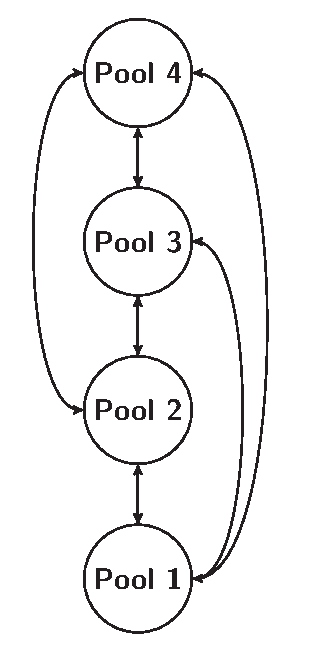
\includegraphics[width=0.25\textheight]{Figure4.eps} % requires the graphicx package
   \caption{A series of connected pools that form the river system used for the second case study. Transitions that ``skip'' pools are possible because fish can move among multiple pools during the course of an annual time step. The model ignores transitions that occur if a fish ends in the same pool it begins in. For example, if a fish starts in Pool 1, swims to Pool 2, and then swims back to Pool 1, the model would not record any transitions for the fish.}
   \label{fig:seriesPool}
\end{figure}



%Do the individuals form or belong to aggregations that affect, and are affected by, the individuals?
%Such collectives can be an important intermediate level of organization in an ABM; examples include social
%groups, fish schools and bird flocks, and human networks and organizations. How are collectives represented? Is
%a particular collective an emergent property of the individuals, such as a flock of birds that assembles as a result
%of individual behaviors, or is the collective simply a definition by the modeler, such as the set of individuals with
%certain properties, defined as a separate kind of entity with its own state variables and traits?

\subsubsection{Observation}

The grass carp population numbers and lengths are the endpoint kept from the model.  

%What data are collected from the ABM for testing, understanding, and analyzing it, and how and
%when are they collected? Are all output data freely used, or are only certain data sampled and used, to imitate
%what can be observed in an empirical study (``Virtual Ecologist'' approach; Zurell et al., 2010)?��

\subsection{Initialization}\label{sec:init}

The initial grass carp population is the initial settings for our model.
This population has three important attributes: size distribution (i.e., ``what lengths are the fish?''), sex distribution, and number.
The transient dynamics of the system are important for the system and can change the behavior of the system.
The initial conditions were not parameterized because the initial release(s) and escape(s) of grass carps into the Great Lakes and Mississippi River Basin are unknown. 
Additionally, the stochastic probability of spawning occurring is an important initial condition, although the model eventually reaches a quasi-stationary distribution.  
We used a lognormal distribution with a mean of log(50) and standard deviation of 0.2 for our population's initial distribution. 


%What is the initial state of the model world, i.e., at time t = 0 of a simulation run? In detail, how
%many entities of what type are there initially, and what are the exact values of their state variables (or how were
%they set stochastically)? Is initialization always the same, or is it allowed to vary among simulations? Are the
%initial values chosen arbitrarily or based on data? References to those data should be provided.

\subsection{Input data}\label{sec:Input}

Grass carp are a highly studied species because of their dual importance as an aquaculture species and invasive species.
In aquaculture, grass carp are an important species for vegetation control \citep{chilton1992biology}. 
In conservation biology and fisheries management, grass carp have large impacts as an invasive species by disrupting native vegetation communities and out-competing native fish \citep{chapman2013first, wittmann2014grass}. 
Because of this, many studies have been conducted that provide specific parameters as well as large-scale synthesis pieces that cover the life-history of the species \citep[e.g.,][]{shireman1983synopsis}.
This rich literature source has provided a source of parameter values for the model (Table \ref{tab:parameterValues}).
In this section, we walk through the different parameters used for the integral projection model.

\begin{table}[htbp]
   \centering
\topcaption{Parameter symbols, names, values, and sources used for grass carp integrated population model. All units are on an annual time step. Lengths are in cm and weights in kg.} % requires the topcapt package
\resizebox{\textwidth}{!}{%
   \begin{tabular}{@{} c lc l c @{}} % Column formatting, @{} suppresses leading/trailing space
      \toprule
%      \multicolumn{2}{c}{Item} \\
%      \cmidrule(r){1-2} % Partial rule. (r) trims the line a little bit on the right; (l) & (lr) also possible
      Symbol   & Name  & Value &  Parameter source \\
      \midrule
       \multicolumn{4}{l}{Length-weight model} \\
\(\alpha_\text{LW}\) & Intercept for  & -4.33 & \citep{wanner2009length}\\
\(\beta_\text{LW}\)   & Slope  & 2.77 & \citep{wanner2009length}\\
 \cmidrule(r){1-4}
 \multicolumn{4}{l}{Growth function, \(G(z, z^\prime)\)} \\
\(a_G\) & Maximum length  &  180 & \citep{USFWS2014grass}\\
\(k_G\)   & Growth rate        & 0.15 & \citep{shireman1983synopsis}\\
\(\sigma_G\)   & Growth \(\sigma\)       & 10 & \citep{shireman1983synopsis}\\
 \cmidrule(r){1-4}
 \multicolumn{4}{l}{Logistic survival function, \(S(z)\)} \\
\(s_\text{min}\) & Minimum survival  & 0.10 & \citep{kirk2003longevity}\\
\(s_\text{max}\) & Maximum survival & 0.90 & \citep{kirk2003longevity}\\
\(\alpha_s\) & Inflection point & 40 & \citep{shireman1978size}\\
\(\beta_s\) & Slope & -5 & \\
 \cmidrule(r){1-4}
  \multicolumn{4}{l}{Density function} \\
\(a\) & Multiplier parameter & 1 & \\
\(b\) & Rate parameter & scenario specific\\
 \cmidrule(r){1-4}
\(e_t\) & Egg transition & \(3\times10^{-3}\) & \\
\cmidrule(r){1-4}
 \multicolumn{4}{l}{Probability of successful spawning and recruitment} \\
\(p_\text{recruit}\) & Probability & \(\text{Beta}(\alpha = 0.25, \beta = 0.25)\)& (P.~Kocovsky, personal observation) \\
\cmidrule(r){1-4}
 \multicolumn{4}{l}{Logistic spawning probability function, \(P_r(z)\)} \\
\(r_\text{min}\) & Min spawning prob & 0 & \citep{shireman1983synopsis} \\
\(r_\text{max}\) & Max spawning prob & 1.0 & \citep{shireman1983synopsis} \\
\(\alpha_r\) & Spawning infection point & 40 & \citep{shireman1983synopsis} \\
\(\beta_r\) & Spawning  slope & -4 & \ \\
 \midrule
 \(e_\text{kg}\) & Eggs produced per kg & \(5\times10^{3}\) & \citep{ashraf1998effects}\\
  \midrule
   \multicolumn{4}{l}{Length distribution of age-1 fish \(J(z)\)} \\
 \(\mu_\text{J}\) & Mean & log(10) & \citep{shireman1983synopsis} \\ 
 \(\sigma_\text{J}\) & Standard deviation & log(2) &   \\ 
   \midrule
   \multicolumn{4}{l}{Sex distribution at birth} \\
  \(p_f\) & Proportion females  & 0.5 &  \citep{shireman1983synopsis} \\ 
  \(p_f\) & Proportion males  & \(1 - p_f\) &  \\ 
      \bottomrule
   \end{tabular} }
   \label{tab:parameterValues}
\end{table}


\subsubsection{Length-weight relationship}

Several studies exist that examine the relationship between length and weight of grass carp \citep[e.g.,][]{dhanze1997biology}.
Most of these relationships are for populations outside of North America in aquaculture settings.
We choose to use the relationship parameterized by \citet{wanner2009length}.
\citet{wanner2009length} examined the length weight relationship for three species of invasive carps in the Missouri River including grass carp.
The study examined carps at two reaches, Gavins Point and Interior Highlands, using a log-log relationship:
\begin{eqnarray}
\text{Log}_{10}\text{weight} = \alpha_{\text{LW}} + \beta_{\text{LW}} \text{Log}_{10}\text{length}  \label{eqn:LW}
\end{eqnarray}
The relationship between log\(_{10}\) length and log\(_{10}\) weight was statistically indistinguishable  between reaches.
We used the relationship estimated for Interior Highlands because it has a lager samples size (\(n=\) 78 versus \(n=33\); Table \ref{tab:parameterValues}).
This data fit the model well (\(r^2 = 0.88\)) for observational field data. 

\subsubsection{Growth-rate}

We assumed that grass carp grew using following a von Bertalanffy curve \citep{bolker2008ecological}
The maximum length of grass carp has been reported to be 150 cm \citep{USFWS2014grass}.
We choose the asymptotic limit in our model, \(a_g\), to be 180 cm, because this causes the maximum length of most grass carp to about 100 cm or less, which is similar to size distributions reported in the literature \citep{shireman1983synopsis,  martyn1986mapping}.
We calculated the annual growth rate, \(k_g\), and standard deviation, \(\sigma_g\), using lengths summarized by \citet{shireman1983synopsis}.
The standard deviation was increased because \citet{shireman1983synopsis} only included means as part of their work.
The standard deviation is on the scale of the length whereas the growth is an annual percentage. 


\subsubsection{Survival}

Many studies of grass carp survival examine rearing the fish in aquaculture conditions \citep[e.g.,][]{stott1973note, kilambi1980food, shelton1981density, cassani1986efficient}.
Fewer studies exist that examine grass carp survival in wild settings \citep{shireman1983synopsis}.
In general, grass carp experience higher mortality at smaller size \citep{shireman1983synopsis}.
At smaller sizes, carp face intraspecific competition and predation risk \citep{shireman1983synopsis}, with carp size being an important limitation to predation in North America \citep{shireman1978size}.
As grass carp grow larger, predation risk decreases and by the time grass carp are longer than 45cm, predation risk decreases greatly \citep{shireman1978size}.

Our model includes  young-of-the-year grass carp survival into the egg transition parameter \(e_t\).
No data exists for this parameter, although the model results are extremely sensitive to the parameter's values. 
Once eggs transition to first-year individuals, survival increases with size.
Grass carp can be a long-lived fish species with individuals living greater than 20 years \citep{shireman1983synopsis}.
A reservoir-based study found annual mortality rates ranging from 22\% to 39\% meaning that 10\% of a cohort could persist for 5 to 9 years \citep{kirk2003longevity}.
For post-egg grass carp, we choose the minimum survival rate to be 10\% and the maximum to be 90\%
The inflection point for the logistic curve was chosen to be 40 cm, which reflects the increase in survival as individuals grow larger. 
The slope parameter was selected because it yields reasonable function behavior.

\subsubsection{Density}

Density affects the ability of grass carp to successfully produce offspring \citep{kilambi1979effects, shelton1981density} and we modeled the effects of density exclusively on off-spring survival. 
The number of carps found in our target system are unknown and we explored this uncertainty with different carrying capacities for the system. 

\subsubsection{Egg production and transition to recruits}

The probability of spawning increases as grass carp increase in size.
The smallest carp have no probability of spawning and we assumed a maximum probability of spawning to be 1.0 \citep{shireman1983synopsis}.
The inflection point was chosen to be 40 cm, which assumes 1/2 of all carp reach sexual maturity by the time they grow to be 40 cm. 
The slope was chose to be -4 for the logistic function. 

The number of eggs produced per female is a function that uses the length-weight function to convert length to weight and then uses the the eggs per kg to calculate the eggs produced by females. 
We used a value of 5,000 egg kg\(^{-1}\) for \(e_\text{kg}\) based upon production and fertilization rates reported by \citet{ashraf1998effects}.

The initial size of recruits was a lognormal distribution with a mean of log(10) and standard deviation of log(2) based upon values reported by \citet{shireman1983synopsis}. 

\subsubsection{Sex ratio}

We assumed a sex ratio of 50\% for the initial population and new recruits because of a paucity of evidence to indicate another ratio \citep{shireman1983synopsis}.
This ratio can be changed through the introduction of YY-males into the population. 
We explored this assumption in our sensitivity analysis. 

%\subsection{Stochastic spawning and recruitment}
%
%Based upon observations from Lake Erie (P.~Kocovsky, personal observation), we choose to model the probability of successful spawning and recruitment during a given year as a beta distribution with \(\alpha = 0.75, \beta=0.75\). 
%This produces a bimodal distribution with mostly boom or bust years (i.e., almost all or none of the population successfully spawns and produces recruits), but allows for some years with partial success. 


\subsection{Submodels}\label{sec:submdl}

\subsubsection{Integral Projection Model}

We modeled the life history of carp using an integral projection model based upon previous work by \citet{Erickson:2017ecomod}. 
Our model  presentation closely followes that of \citet{Erickson:2017ecomod}.
Recent work provides overviews, introductions, and tutorials of integral projection models for readers who are unfamiliar with their basic application \citep[e.g.,][]{ellner2006integral, ramula2009integral, Ellner:2010IPM, merow2014advancing}.
The continuous-length distribution of individuals within populations form the basic foundations of the model (Figure \ref{fig:cMap}).
We model the length of individuals (\(z\)) within the population through discrete time (\(t\)).
The variable \(z\) ranges over an interval of possible lengths \(\Omega\), with considerations for unintentional eviction \citep{williams2012avoiding}.
Our specific time step differs between case studies, reflecting the different amounts of biological data for the case studies.
By default, we include 2 fixed population sex-classes within the model: females \(P_\text{f}(z,t))\) and males \(P_\text{m}(z, t)\) of size \(z\) at time \(t)\). 
Our model includes the option to add additional sex-classes such as YY-males \citep{Erickson:2017ecomod} or genetically modified sterile individuals \citep{knols2006gm} or ignore sex-structure within the populations.
We include some of these variations within this paper. 


\begin{figure}[htbp]
	\centering
	\includegraphics[width = 0.5\textwidth]{../../manuscript/Figure2.eps} 
	   \caption{Conceptual map of carp life history. \(p_f\) is the proportion of female recruits and \(p_m\) is the proportion of male recruits. By definition, \(p_f + p_m = 1\).  The recruitment kernel (\(F(z, z^\prime)\)) is defined in Equation \ref{eqn:Fec}, where \(z\) is size at the current time, \(t\) and \(z^\prime\) is the size at the next time step \(t+1\). The growth/survival kernel (\(M (z, z')\)) is defined in Equation \ref{eqn:growMat}.  Growth/maturation is the annual increase in fish length including the survival. Recruitment is the successful spawning and development of eggs to produce age-1 fish. Recruitment does not occur from females until they become of sufficient length. Figure is reprinted from \citet{Erickson:2017ecomod}  and is in the public domain because it was created by a US Government Employee as part of his official duties.}
   \label{fig:cMap}
\end{figure}

An integral gives the total population size of female carp at each time step \(t\)
\begin{equation*}
||P_{\text{f}}(\cdot, t)|| = \int_{\Omega}P_{\text{f}}(z, t) dz,
\end{equation*}
with similar equations existing for males and other possible sex classes (e.g., sterile males or YY-males).
Using matrix population models, one ``projects'' the population size and distribution from one time step to the next by multiplying a population vector with a matrix.
Using integral projection models, one ``integrates'' the integral kernel (i.e., the function from one time step to the next) \(K(z,z')\) to calculate the population size through time: 
\begin{equation*}
P(z', t+1) = \int_{\Omega} (K(z, z')P(z, t))\; dz
\end{equation*}
for each time \(t\). 
Note that if \(z\) is the current length at time \(t\), then \(z^\prime\) is the length at time \(t+1\).
The kernel often can be split into two kernels: a kernel for recruitment/fecundity and a kernel for growth and maturation \citep{ellner2006integral}.  
Additionally, we include immigration, \(I(z)\), and emigration, \(E(z)\), kernels modeling connections among subpopulation as a function of fish size.
These terms include both movement mappings and survival  (i.e., they indicate the probability of a fish both moving between nodes and surviving the move).
Non-moving fish have a different survival function.
The growth and maturation kernel, \(M\), models how fish grow in length as a function of time and includes both survival, \(S(z)\), and growth, \(G(z, z^\prime)\). 
\begin{eqnarray}
M(z, z^\prime) = S(z) G(z, z^\prime).\label{eqn:growMat}
\end{eqnarray}
We used a four-parameter logistic function for survival:
a minimum survival rate, \(s_\text{min}\); 
a maximum survival rate, \(s_\text{max}\);
an intercept parameter, \(\alpha_s\); and 
a slope parameter, \(\beta_s\) \citep{bolker2008ecological}:
\begin{eqnarray}
S(z) = s_\text{min} + \frac{s_\text{max} - s_\text{min}}{ 1 + e^{\beta_s (\log(z) - \log(\alpha_s))}}. \label{eqn:surlog}
\end{eqnarray}
We modified and derived a von Bertalanffy function to model growth.
First, we took the derivative of the length with respect to length (i.e., how length changes as a function of length) because the von Bertalanffy function usually denotes the relationship between time and length.
Second, we assumed the function was centered around a modified normal distirbution. 
We created a mapping between current size at time \(t\) (\(z\)) and size at the next time step \(t+1\) (\(z^\prime\)).
Our new function included two parameters for the modified von Bertalanffy equation: \(k_g\) and \(a_g\), and a standard deviation \(\sigma_g\):
\begin{eqnarray}
G(z, z^\prime) &=&  \text{Prob}(z^\prime | z, k_g, a_g, \sigma_g) = \text{Normal PDF}((1 - k_g) z + k_g  a_g , \sigma_G).\label{eqn:Growth}
\end{eqnarray}

Our fecundity/recruitment kernel, \(F\), is a function of the probability of 
an egg transitioning to become a recruit, \(e_t\);
the probability of females surviving from the previous year, \(S(z)\);
the probability of females spawning, \(P_r(z)\);
the number of eggs produced per female, \(Egg(z)\); and 
the initial recruit length distribution, \(J(z^\prime\)):
\begin{eqnarray}
F(z, z^\prime) &=& e_t S(z) P_r(z) Egg(z) J(z).\label{eqn:Fec}
\end{eqnarray}
\(S(z)\) and \(P_r(z)\) are both logistic functions, while
\(Egg(z)\) is the function of eggs produced by fish based upon her length, using the length-weight relationship. 
The input, female fish length \(z\), is converted to biomass based upon the relationship between weight and length from \cite{wanner2009length}:
\begin{eqnarray}
\text{log}_{10} (\text{biomass}) = \alpha_{\text{lw}} + \beta_\text{lw}\text{log}_{10} (z)\label{eqn:LW},
\end{eqnarray}
which is integrated for the entire female population.
This is then multiplied by the eggs produced per kg of female (\(e_\text{kg}\)).  
The minimum probability of spawning is \(r_\text{min}\);
the maximum probability of spawning is \(r_\text{max}\);
the probability of spawning  intercept parameter is \(\alpha_r\);  and
the probability of spawning slope parameter is \(\beta_r\).
The recruit length distribution is the length distribution of recruits and is a log-normal distribution with mean \(\mu_J\) and standard deviation \(\sigma_J\).
The egg transition probability to recruits includes the eggs fertilization, survival, and recruitment to age-1 fish.

The proportion of spawning and successful recruitment during a given year, \(p_\text{recruit}\)  depends on population density, \(d\).  
The effect of density is calculated using the total biomass of carp (i.e., the sum of the weight for all individuals carp), using Equation \ref{eqn:LW}.  
This biomass calculation is then used in a negative exponential function to calculate the decrease in fecundity caused by grass carp density:
\begin{eqnarray}
d  = a e^{-b \text{biomass}}.
\end{eqnarray}
These terms are combined to make the (now density-dependent) male kernel:
\begin{eqnarray}
P_\text{male}(z', t + 1) = \int_\omega (M(z,z') P_\text{male}(z, t) + F(z,z') P_\text{female}(z, t) p_{m}; d \; p_\text{recruit} + I(z)  - E(z)) \; dz.
\end{eqnarray}
The female year-to-year projection is similar to the male kernel:
\begin{eqnarray}
P_\text{female}(z', t + 1) = \int_\omega (M(z,z') P_\text{female}(z, t) + F(z,z') P_\text{female}(z, t) p_{f}\; d \; p_\text{recruit} + I(z)  - E(z)) \; dz.\label{eqn:femaleEQN}
\end{eqnarray}

Our model makes an important assumptions about grass carp and the impacts of sex.
Our model assumes that XY-males and females survive, grow, and are produced at the same rate.
We made these assumptions because data do not exist for the growth and survival of each sex individually.
For models with sterile males, we either assumed the sterile males had the same survival as normal males or had reduced survival. 
This was done to explore potential modified organisms as a control tool.

For scenarios with harvest, we assumed harvest either had a uniform distribution across size or a 
4-parameter logistic equation (similar to Equation \ref{eqn:surlog}), but with different parameter values.
The logistic harvest model allowed for larger fish to have a higher probability of harvest because these fish are easier to harvest. 


\subsubsection{Network-node model}


 \citet{Taylor:2010} presented a network-node framework for examining populations dynamics through space that could readily be adapted to also include time \citep[e.g.,][]{Erickson:2014, Wiederholt:inreview, erickson2016effects}.
This framework describes nodes that are connected by edges to form a network. 
The framework follows the migratory path (i.e., the set of all nodes and edges) a group of individuals use through time.
The network model assumes groups do not change paths, allowing for paths to go extinct, but not be re-populated.
 \citet{Taylor:2010} originally considered species with forced migration (e.g., migratory birds with non-overlapping summer and winter habitat), but their framework readily generalizes include partial migration (e.g., some groups do not migrate) and no migration (e.g., the model does not impose migratory dynamics) \citep{erickson:2017}. 
 We further generalize their framework to use IPMs within each node. 
 Our model can include ``time periods'' such as seasons (e.g., summer, winter) or within-year discretizations of time. 
 These time periods do not need to be the same length (e.g., time period 1 could be 2 months and time period 2 could be 10 months), but the units within each time period must have consistent units (e.g., events per 2 months for all parameter in time period 1).
 
Broadly, we attempted to avoid using formal notation for nodes and edges unless absolutely necessary because it complicates the equations.
When necessary, we used forward subscripts for locations (e.g., parameter or variable \(X\) for node 1 would be \(\prescript{}{1}{X}\)) and edges (e.g.,  parameter or variable \(X\) for the edge between nodes 2 and 3 would be \(\prescript{}{2,3}{X}\)).
We were able to avoid this notation in our code by using an object-orientated programing approach.


\stopcontents[sections]

\section{Data evaluation}\label{sec:dev}

\textbf{This TRACE element provides supporting information on:} The quality and sources of numerical and qualitative data used to parameterize the model, both directly and inversely via calibration, and of the observed patterns that were used to design the overall model structure. This critical evaluation will allow model users to assess the scope and the uncertainty of the data and knowledge on which the model is based.

\textbf{Summary:}
\begin{verse}
\textbf{
Our model used published parameter values, as described in \S \ref{sec:Input}.
We intentionally present our model as theoretical, hence it matches no exact population.
However, our broad, qualitative findings agree with other another Asian carp population models developed for the Illinois River System (D.~Glover, personal observation).
We discuss limitation of our data in this section and the impact of the limitations on our model.
We also discuss how our data is similar to a published study that examined length through time.
}
\end{verse}

Portions of this section could be redundant with \S \ref{sec:Input}.
We therefore focus on the quality of data within this section.
Grass carp are a well studied species because of their importance in aquaculture and their impact as an invasive species.
We therefore had a large range of literature to draw upon.
First, we discuss the limitations of lacking a relative population estimate for our species.
Second, we compare our model outputs of length to those from a study published in the literature.

Broadly, one of the largest hurdles to our model and any population modeling effort used to guide resource is density, how it limits population growth, and estimating these two effects.
We assumed only recruitment was impacted by density, a seemingly reasonable assumption for this system and one made another modeling team examining this system (D.~Glover, personal observation).
However, scaling the population size is difficult because no reliable population estimates exist for grass carp populations in systems such as Lake Erie or the Mississippi River system and its tributaries (e.g., Illinois River, Missouri River).  

Qualitatively, our model outputs were similar to length distributions reported by \citet{martyn1986mapping}.
\citet{martyn1986mapping} sought to evaluate grass carp a control for aquatic weeds.
As part of their methods, 270,000 grass carp were socked into an 8,100 ha reservoir located near Houston, TX over 2 years. 
The length of the fish were recored prior to release and also twice during the study as part of rotenone based sampling.
The fish lengths for distinct modes for each release period \citep[Figure 11 in][]{martyn1986mapping}.
Additionally, these frequency plots of length are qualitatively similar to our model's outputs. 

Quantitively, we would expect our model to have a slower growth rate than the carp observed by \citet{martyn1986mapping}.
\citet{martyn1986mapping} examined carp in the southern United States, near Houston, TX, which is a sub-tropical region.
Our model is for Lake Erie, which is a temperate, continental climate region.
Although we did not parameterize our model with parameters specific to Lake Eric, our parameter sources were from temperate regions of the former USSR. 
This qualitative agreement lends additional support to our model. 


\section{Conceptual model evaluation}
\textbf{This TRACE element provides supporting information on:} The simplifying assumptions underlying a model's design, both with regard to empirical knowledge and general, basic principles. This critical evaluation allows model users to understand that model design was not ad hoc but based on carefully scrutinized considerations. 

\textbf{Summary:}
\begin{verse}
\textbf{
Our model is based upon the life history of carp.
Although specifically designed for grass carp, the model should work for any species of carp.
More broadly, our model should apply to any species that lives in discrete habitat patches.
Our implementation of the network-node model and IPM allow for life- and age-stages to be included within the model as well. 
} 
\end{verse}

Grass carp, like most species of fish, experience asymptotic growth and continue to grow throughout their life  \citep{lagler1962john}.
Individual females also produces more eggs as they increase and larger individuals are more likely to spawn than smaller individuals.
Additionally, larger individuals of both have higher survival rates than smaller individuals \citep{shireman1983synopsis}. 
These characteristics create a species that would be well described by an integral projection model \citep{ellner2006integral, ramula2009integral, merow2014advancing}.  

We created an integral projection model that matches the life history of grass carp (Figure \ref{fig:cMap}).
The fish become recruits that survive the first year.
Then, the individuals grow. 
Following a logistic curve, the probability of females spawning and producing recruits increases with their size. 
Similarly, survival follows a logistic curve with longer individuals being more likely to survive than smaller individuals.

We also allow the model to include modified groups of fish such as sterile males (included in the case study) or yy-males \citep[previously described in][]{Erickson:2017ecomod}.
The sterile males decrease the recruitment of viable individuals.
The goal of management strategy is to cause a population collapse by stopping recruitment. 
It has been used as a method for mosquito control \citep[e.g.,][]{benedict2003first}.
We compared two different release scenarios for the modified organisms.
First, we assumed the modified organisms were the same as normal males.
Second, we explored using modified organisms that had half maximum survival rate as normal males.
The sterile males decrease the sex ratio of the offspring and skew it towards male.
The goal of this management strategy is to decrease the population growth rate by decreasing the number of females \citep{schill2016production}. 
These individuals are assumed to be the same demographically as XY-males for one set of scenarios and have decreased survival for a second set of scenarios. 
Although no YY-males or sterile have yet been created, triploid carps have been released to control vegetation.
These individuals appear to have similar lifespans based upon research from reservoirs in the southeastern United States \citep{kirk2003longevity} and anecdotal evidences from pond owners who have released them (\url{http://forums.pondboss.com/ubbthreads.php?ubb=showflat&Number=146930}).

Our model also allows other control tools to be included.
Proportional harvest (e.g., 10\% of the population) can be included within the model.
The model also allows tools such barriers to be examined.
Barriers work by decreasing carp movement among nodes.


\begin{figure}[htbp]
	\centering
	\includegraphics[width = 0.4\textwidth]{../../../Figure/FlowChart.pdf} 
	   \caption{Conceptual map of grass carp life history. \(p_f\) is the proportion of recruits who are female and \(p_m\) is the proportion who are male. By definition, \(p_f + p_m = 1\).  Our model seeks to alter this ratio through the introduction of YY-males. Growth/maturation is the annual increase in fish length. Recruitment is the successful spawning and development of eggs to produce age-1 fish. Recruitment does not occur from females until they increase in length.}
   \label{fig:cMap}
\end{figure}


\section{Implementation verification}\label{sec:IpVer}
\textbf{This TRACE element provides supporting information on:} The simplifying assumptions underlying a model's design, both with regard to empirical knowledge and general, basic principles. This critical evaluation allows model users to understand that model design was not ad hoc but based on carefully scrutinized considerations. 

\textbf{Summary:}
\begin{verse}
\textbf{ 
We build the model using Python.
We included formal unit testing and version control as part of our model building.
We also included non-unit testing to check our code's plotting function.
Additionally, we created a Universal Modeling Language (UML) diagram of our model's code.}
\end{verse}

We build our model using unit testing, using the \texttt{unittest} module in Python.
These tests ensure functions behave as expected and provide coverage of most of the model's code.
We have included this test code as part of our \texttt{git} repository.  
We also ensured our mesh size did not gain or lose fish \citep{williams2012avoiding}.  
We also created a Universal Modeling Language (UML) diagram of our model's code design. 

\section{Model output verification}

\textbf{This TRACE element provides supporting information on:} (1) how well model output matches observations and (2) how much calibration and effects of environmental drivers were involved in obtaining good fits of model output and data. 

\textbf{Summary:}
\begin{verse}
\textbf{
Our model was unable to be formally parameterized. 
However, we qualitatively compared our model's outputs to existing data and discuss this realism. 
}
\end{verse}

We were unable to formally parameterize our model. 
We were able to qualitatively compare our results to a study by \citet{martyn1986mapping} who examined the length distributions of grass carp following their release into a reservoir.
Additionally, \S \ref{sec:IpVer} aggress with observations that would be expected based upon first principles of fish population dynamics. 

\section{Model analysis}

\textbf{This TRACE element provides supporting information on:} (1) how sensitive model output is to changes in model parameters (sensitivity analysis), and (2) how well the emergence of model output has been understood. 

\textbf{Summary:}
\begin{verse}
\textbf{
We did not conduct formal sensitivity analysis within this project.
However, we did examine how changing treatments impacted the population dynamics of the system.
We plan formal sensitivity analysis as part of future research on this model.
}
\end{verse}

\section{Model output corroboration}

\textbf{This TRACE element provides supporting information on:}  How model predictions compare to independent data and patterns that were not used, and preferably not even known, while the model was developed, parameterized, and verified. By documenting model output corroboration, model users learn about evidence which, in addition to model output verification, indicates that the model is structurally realistic so that its predictions can be trusted to some degree. 

\textbf{Summary:}
\begin{verse}
\textbf{
We were unable to formally corroborate our model to any datasets.
We discuss a qualitative corroboration to a previously study and why existing datasets do not allow for corroboration.
}
\end{verse}

No datasets exist that examine our system or a similar system through time.
Qualitatively, our results were similar \citet{martyn1986mapping} as noted in \S \ref{sec:dev}.
In both our model and their system system, he population of carps grows in length through time. 
However, robust field observations of large-scale grass carp invasions are sparse. 


%% If using natbib, you need a style and file for your bibliography
\bibliographystyle{elsarticle-harv}
\bibliography{/Users/rerickson/Documents/bibFiles/allBib.bib}

\end{document}